\documentclass[a4paper]{article}
\usepackage[utf8x]{inputenc}
\usepackage[T1]{fontenc}
\usepackage[MeX]{polski}
\usepackage{amssymb}
\usepackage{graphicx}
\usepackage{fancyhdr}
\usepackage{lastpage}
\usepackage{xcolor}
\usepackage{color, colortbl}
\usepackage{hyperref}
\definecolor{tableofcontents}{RGB}{0, 0, 0}
\hypersetup{
    colorlinks=true,
    urlcolor=blue,
    linkcolor=tableofcontents,
}


\pagestyle{fancy}
\fancyhf{}
\cfoot{ \thepage \hspace{1pt} / \pageref{LastPage}}
\lhead{Sprawozdanie ko\'ncowe}
\rhead{\texttt{War Of Tanks}}


\begin{document}

\begin{titlepage}
	\begin{center}
		\vspace*{5cm}

	        \Huge
        	\textbf{Sprawozdanie ko\'ncowe}

        	\vspace{1cm}
	        \Huge
        	\texttt{War Of Tanks}

    		\vspace{1.5cm}

	        \large
		    Aleksandra Michalska, Natalia Olszewska

        	\vfill

	        \vspace{3cm}

		\large 08.06.2021
	\end{center}
\end{titlepage}

\tableofcontents

\newpage


\section{Informacje og\'olne}

\subsection{O dokumencie}
\quad Dokument jest podsumowaniem pracy nad projektem gry \texttt{WarOfTanks}. 
Koresponduje z dokumentami \textit{"Specyfikacja funkcjonalna"} oraz \textit{"Specyfikacja implementacyjna"}.

\subsection{O programie}
\quad Program jest przeznaczony dla dw\'och u\.zytkownik\'ow korzystaj\k{a}cych z jednego urz\k{a}dzenia. Ich zadaniem jest strzelanie do spadaj\k{a}cych kom\'orek przy pomocy poruszaj\k{a}cych si\k{e} czo\l{}g\'ow.
Wygrywa ten u\.zytkownik, kt\'ory uzyska wi\k{e}ksz\k{a} liczb\k{e} punkt\'ow na koniec gry.

\subsection{\'Srodowisko implementacyjne i funkcjonalne}
\quad Program zosta\l{} zaimplementowany w j\k{e}zyku programowania \textbf{Java 1.8} w systemie operacyjnym \textbf{Windows 10}. 

W celu kontroli wersji zosta\l{} u\.zyty \textbf{Projektor EE} (system kontroli wersji Politechniki Warszawskiej). 

W potrzebie uzyskania wi\k{e}cej informacji implementacyjnych patrz \textit{"Specyfikacja implementacyjna" punkt 1}.

\section{Zmiany w funkcjonowaniu programu}

\subsection{Uruchomienie programu}
\quad Uruchomienie programu mo\.ze odbywa\'c si\k{e} na dwa sposoby:
\begin{enumerate}
    \item przy pomocy odpowiednich program\'ow (np. IntelliJ IDEA, NetBeans)
    \item przy pomocy konsoli systemowej. W tym sposobie nale\.zy przej\'s\'c do katalogu \texttt{/out/production/Tanks game} i z tego poziomu u\.zy\'c polecenia:
    \begin{center}
        java frames.MainOfWar
    \end{center}
    
\end{enumerate}

\subsection{Domy\'slne warto\'sci paramentr\'ow programu}
\quad W celu poprawy funkcjonowania programu, zosta\l{}y ustalone nowe domy\'slne warto\'sci parametr\'ow programu (patrz \textit{Tabela \ref{table:ta}}).

\begin{table}[ht]
\centering
    \renewcommand{\arraystretch}{1.3}
    \begin{tabular}{|c|c|}
    \rowcolor{lightgray}
        \hline
        parametr&warto\'s\'c \\
        \hline
        v1&30\\
        \hline
        dv1&5\\
        \hline
        v2&60\\
        \hline
        dv2&10\\
        \hline
        t1&30\\
        \hline
        t2&10\\
        \hline
        t3&3\\
        \hline
\end{tabular}
\quad
    \begin{tabular}{|c|c|}
    \rowcolor{lightgray}
        \hline 
        parametr&warto\'s\'c\\
        \hline
        x1&7\\ 
        \hline
        p1&3\\
        \hline
        r1&20\\
        \hline
        dr1&5\\
        \hline
        h1&70\\
        \hline
        dh1&5\\
        \hline
\end{tabular}
\color{lightgray}\caption{Domy\'slne warto\'sci parametr\'ow programu}
\label{table:ta}
\end{table}

\subsection{Ograniczenia parametr\'ow programu}
\quad W zwi\k{a}zku ze zmian\k{a} domy\'slnych warto\'sci parametr\'ow programu, zosta\l{}y zmienione ich ograniczenia (patrz \textit{Tabela \ref{table:ograniczenia}}).

\begin{table}[ht]
\centering
    \renewcommand{\arraystretch}{1.5}
    \begin{tabular}{|c|c|}
    \rowcolor{lightgray}
        \hline
        parametr&ograniczenie \\
        \hline
        v1& \(10 \leqslant v1 \leqslant 50\)\\
        \hline
        dv1& \(0 \leqslant dv1 \leqslant 25\)\\
        \hline
        v2& \(5 \leqslant v2 \leqslant 35\)\\
        \hline
        dv2& \(0 \leqslant dv2 \leqslant 20\)\\
        \hline
        t1& \(30 \leqslant t1 \leqslant  180\)\\
        \hline
        t2& \(5 \leqslant t2 \leqslant 40\)\\
        \hline
        t3& \(3 \leqslant t3 \leqslant 15\)\\
        \hline
\end{tabular}
\quad
    \begin{tabular}{|c|c|}
    \rowcolor{lightgray}
        \hline 
        parametr&ograniczenie \\
        \hline
        x1& \(0 \leqslant x1 \leqslant 25\)\\ 
        \hline
        p1& \(1 \leqslant p1 \leqslant 9\)\\
        \hline
        r1& \(5 \leqslant r1 \leqslant 25\)\\
        \hline
        dr1& \(2 \leqslant dr1 \leqslant 10\)\\
        \hline
        h1& \(20 \leqslant h1 \leqslant 70\)\\
        \hline
        dh1& \(1 \leqslant dh1 \leqslant 10\)\\
        \hline
\end{tabular}
\color{lightgray}\caption{Ograniczenia parametr\'ow programu}
\label{table:ograniczenia}
\end{table}

\subsection{Plik konfiguracyjny}
\quad Przekazanie pliku konfiguracyjnego do programu odbywa si\k{e} przez menu \\ \texttt{Add File}.

W przypadku podania (w pliku konfiguracyjnym) nieistniej\k{a}cych parametr\'ow programu lub nieprawid\l{}owych warto\'sci parametr\'ow programu, zostaj\k{a} one pomini\k{e}te i u\.zytkownik nie jest informowany o \.zadnych b\l{}\k{e}dach. Do programu zostaj\k{a} przekazane tylko te warto\'sci parametr\'ow, kt\'ore uda\l{}o si\k{e} poprawnie odczyta\'c, a pozosta\l{}e zostaj\k{a} przypisane jak opisano w sekcji \textit{"Domy\'slne warto\'sci parametr\'ow programu"}. 

Przyk\l{}adowo, podanie nast\k{e}puj\k{a}cych danych w pliku konfiguracyjnym:

\begin{center}
\texttt{\textbf{-nieistniej\k{a}cy 8 -samParametr -v1 z\l{}aWarto\'s\'c -h1 60}}    
\end{center}

skutkuje zmian\k{a} tylko pocz\k{a}tkowej wysoko\'sci kom\'orek na 60 pikseli.

\subsection{Panel gry}
\subsubsection{Ruch czo\l{}gu}
\quad Z powodu kwesti implementacyjnych zosta\l{} zmieniony spos\'ob ruchu czo\l{}gu dla gracza po prawej stronie (niebieski czo\l{}g):
\begin{itemize}
    \item[$\diamond$] ruch w g\'or\k{e}: klawisz \textbf{$\uparrow$}
    \item[$\diamond$] ruch w d\'o\l{}: klawisz \textbf{$\downarrow$}
    \item[$\diamond$] obr\'ot lufy w g\'or\k{e}: klawisz \textbf{$\rightarrow$}
    \item[$\diamond$] obr\'ot lufy w d\'o\l{}: klawisz \textbf{$\leftarrow$}
\end{itemize}

\subsection{Interface gry}
\subsubsection{Pocz\k{a}tkowy ekran}
\quad Ostateczny ekran pocz\k{a}tkowy zawiera 4 przyciski: 
\begin{itemize}
    \item \textbf{START} rozpoczynaj\k{a}cy gr\k{e}
    \item \textbf{HELP} wy\'swietlaj\k{a}cy zasady gry
    \item \textbf{ADD FILE} wy\'swietlaj\k{a}cy okno do za\l{}\k{a}czenia pliku konfiguracyjnego
    \item \textbf{RESET} resetuj\k{a}cy dane wprowadzone za pomoc\k{a} pliku konfiguracyjnego
\end{itemize}

\begin{figure}[ht]
    \centering
    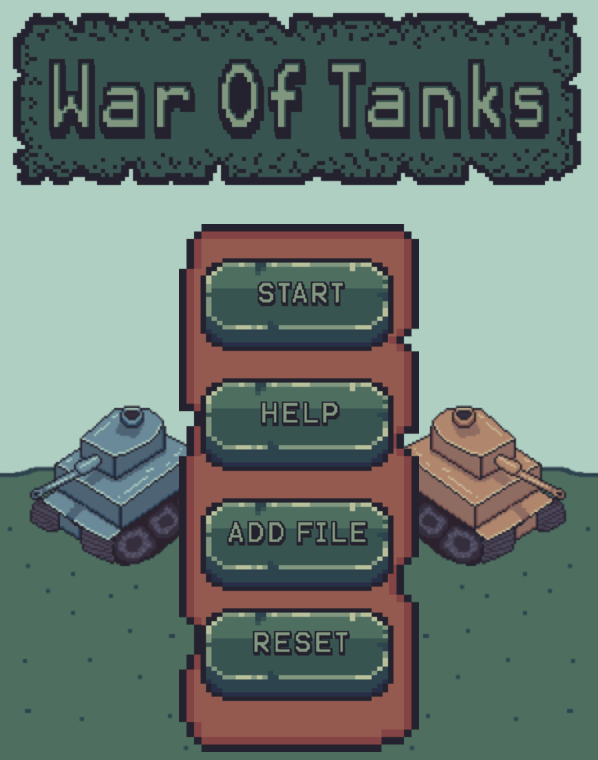
\includegraphics[scale=0.55]{start.png}
    \color{lightgray}\caption{Pocz\k{a}tkowy ekran}
    \label{fig:start}
\end{figure}

\subsubsection{Okno za\l{}\k{a}czania pliku konfiguracyjnego}
\quad Po naci\'sni\k{e}ciu przycisku \textbf{ADD FILE} wy\'swietla si\k{e} okno, w kt\'orym u\.zytkownik mo\.ze wybra\'c plik z danymi.

\begin{figure}[ht]
    \centering
    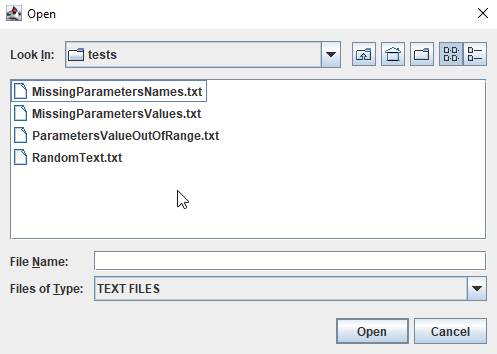
\includegraphics[scale=0.6]{conf.png}
    \color{lightgray}\caption{Okno za\l{}\k{a}czania pliku konfiguracyjnego}
    \label{fig:conf}
\end{figure}

\subsubsection{Ekran gry}
\quad Rozmieszczenie paneli na ekranie gry pozosta\l{}o niezmienione. Ostateczny wygl\k{a}d ekranu gry przedstawiony jest na Rysunku \ref{fig:game}.

\begin{figure}[ht]
    \centering
    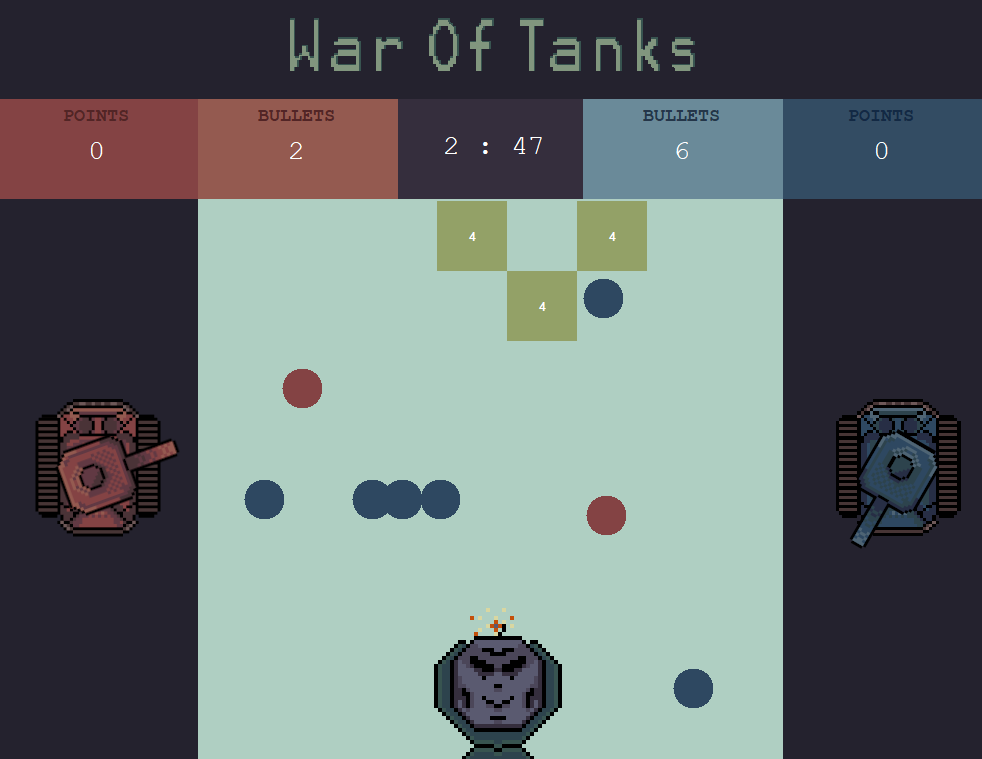
\includegraphics[scale=0.4]{game.png}
    \color{lightgray}\caption{Ekran gry}
    \label{fig:game}
\end{figure}

\subsubsection{Okno zasad gry}
\quad Po naci\'sni\k{e}ciu przycisku \textbf{HELP} wy\'swietla si\k{e} okno, w kt\'orym u\.zytkownik mo\.ze przeczyta\'c zasady gry.

\begin{figure}[ht]
    \centering
    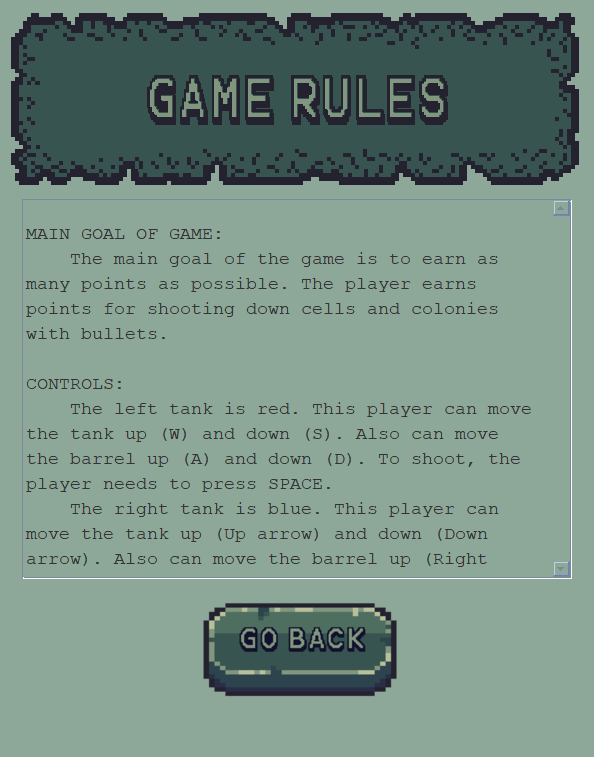
\includegraphics[scale=0.5]{rules.png}
    \color{lightgray}\caption{Okno zasad gry}
    \label{fig:rules}
\end{figure}


\section{Zmiany w implementacji}

\subsection{Diagram klas}

\quad Ze wzgl\k{e}du na zmiany implementacyjne w klasach zosta\l{} zmieniony diagram klas. Z przyczyn wizualnych jest on dost\k{e}pny pod danym \href{https://drive.google.com/file/d/1BycxHSp0vN6H3-6hj7EW1VBEZAAbxgBE/view?usp=sharing}{adresem}.

\subsection{Rezygnacja z element\'ow}

\quad Z powodu niewystarczaj\k{a}cej ilo\'sci czasu komponent \textit{SettingsFrame}, wraz z pod\l{}\k{a}czeniem muzyki do projektu, nie zosta\l{} zaimplementowany.

\subsection{Nowe rozwi\k{a}zania}

\subsubsection{Tank, Body, Barrel}
\quad Zamiast utworzenia dw\'och osobnych klas dla prawego i lewego czo\l{}gu, zosta\l{}a utworzona jedna.
Wykorzystuje ona dwie klasy, ponownie zaimplementowane w pojedyncze, \textit{Body} i \textit{Barrel}.
Przy tworzeniu nowego obiektu typu \textbf{Tank} nale\.zy poda\'c liter\k{e} 'r' lub 'l' odpowiadaj\k{a}c\k{a} stronie czo\l{}gu do utworzenia.

Pozwoli\l{}o to zapobiec powtarzaniu si\k{e} prawie tego samego kodu w celu utworzenia dw\'och obiekt\'ow.

\subsubsection{Colony}
\quad Zast\k{e}pczo do tworzenia jednej klasy abstrakcyjnej i z niej czterech osobnych klas kolonii, zosta\l{}a utworzona klasa generuj\k{a}ca wszelkie mo\.zliwe rozstawienia koloni w siatce 3 na 3.

\subsubsection{SettingImages}
\quad Z powodu du\.zej liczby grafik u\.zytych do projektu zosta\l{}a utworzona klasa \textit{SettingImages}, kt\'ora pobiera grafiki z odpowiednich katalog\'ow i zwraca ich zawarto\'sci w odpowiednich metodach.


\subsubsection{W\k{a}tki}
\quad Program zosta\l{} podzielony na kilka niezale\.znych w\k{a}tk\'ow odpowiadaj\k{a}cych pewnym elementom. Zaliczaj\k{a} si\k{e} do nich:
\begin{itemize}
    \item[$\diamond$] poruszanie czo\l{}giem lewym,
    \item[$\diamond$] poruszanie czo\l{}giem prawym,
    \item[$\diamond$] strzelanie czo\l{}g\'ow,
    \item[$\diamond$] zmiana parametr\'ow. 
\end{itemize}

\subsubsection{ConfFrame}
\quad Do cel\'ow za\l{}\k{a}czenia pliku konfiguracyjnego zosta\l{}a utworzona klasa \textit{ConfFrame}.
Odbiera ona parametry i przetwarza ich zawarto\'s\'c oraz poprawno\'s\'c, modyfikuj\k{a}c przy tym odpowiednio obiekt \textbf{ConfObject} towrzysz\k{a}cy rozgrywce.

\subsection{Zmiany}

\subsubsection{StartFrame}

\quad Zamiast jednej klasy \textit{StartFrame} jej zawarto\'s\'c zosta\l{}a rozdzielona na kilka:
\begin{itemize}
    \item[$\diamond$] \textit{StartPanelTitle} - wy\'swietla tytu\l{} gry w panelu startowym,
    \item[$\diamond$] \textit{StartPanelBackground} - wy\'swietla t\l{}o gry w panelu startowym.
    \item[$\diamond$] \textit{StartPanelButtons} - wy\'swietla panel przycisk\'ow i odpowiada za ich funkcjonowanie,
    \item[$\diamond$] \textit{StartFrame} - odpowiada za wy\'swietlenie ramki panelu startowego. 
\end{itemize}

\subsubsection{HelpFrame}
\quad Do klasy \textit{HelpFrame} zosta\l{}y dodane dwie pomocnicze klasy:
\begin{itemize}
    \item[$\diamond$] \textit{HelpPanelTitle} - wy\'swietla tytu\l{} w panelu pomocy,
    \item[$\diamond$] \textit{GoBackButton} - wy\'swietla przycisk powrotu do panelu startowego.
\end{itemize}

\subsubsection{GameFrame}
\quad Do klasy \textit{GameFrame} zosta\l{}a dopisana pomocnicza \textit{GameTimer}. Odpowiada ona za wykonanie zrzutu ekranu po zako\'nczeniu gry oraz pokazaniu zwyci\k{e}zcy. Wy\'swietla r\'ownie\.z czas danej rozgrywki.

\subsubsection{TankPanel, CellsPanel}
\quad Z klasy \textit{GameFrame} zosta\l{}a wyodr\k{e}biona g\l{}\'owna struktura rozgrywki.
Cz\k{e}\'s\'c zale\.zna od graczy zosta\l{}a zaimplementowana w klasie \textit{TankPanel}. To w\l{}a\'snie tam znajduj\k{a} si\k{e} w\k{a}tki odpowiadaj\k{a}ce poruszaniu i strzelaniu czo\l{}g\'ow.
Rozgrywka od drugiej strony zosta\l{}a umieszczona w \textit{CellsPanel}. W\l{}a\'snie tam generuj\k{a} si\k{e} losowo kom\'orki i kolonie. 

\section{Przeprowadzone testy}

\quad Testy zosta\l{}y podzielone na kilka proces\'ow.

Pierwszymi by\l{}y testy poprzez uruchomienia. Sprawdzanie na pierwszy i drugi rzut oka, czy program wykonuje si\k{e} tak jak powinien. Dotyczy\l{}y one r\'ownie\.z likwidacji ostrze\.ze\'n.

Nast\k{e}pnym procesem by\l{}o dostosowanie projektu do uruchomienia w r\'o\.znych \'srodowiskach. Testy zosta\l{}y przeprowadzone w kompilatorze \textbf{Intellij Idea Project}, terminalu \'srodowiska Windows CMD oraz w terminalu \'srodowiska Linuxa.

Przed podej\'sciem do test\'ow ostatecznych program zosta\l{} przetestowany wzgl\k{e}dem minimalnych i maksymalnych obci\k{a}\.ze\'n oraz warto\'sci parameter\'ow wej\'sciowych.

Ostatnim krokiem by\l{}o przeprowadzenie test\'ow jednostkowych JUnit. W tej cz\k{e}\'sci uwaga zosta\l{}a po\'swi\k{e}cona badaniu poprawno\'sci pojedynczych metod. Zalicza\l{}y si\k{e} do nich m.in:
\begin{itemize}
    \item[$\diamond$] \textit{decreaseBombPoints} - z klasy \textbf{Bomb},
    \item[$\diamond$] \textit{setBulletCoordinate} - z klasy \textbf{Bullet},
    \item[$\diamond$] \textit{changeCellSide} - z klasy \textbf{CellsPanel},
    \item[$\diamond$] \textit{increaseCellPoints} - z klasy \textbf{Cell},
    \item[$\diamond$] \textit{decreaseCellPoints} - z klasy \textbf{Cell},
    \item[$\diamond$] \textit{getIsAlone} - z klasy \textbf{Cell},
    \item[$\diamond$] \textit{getWhichColony} - z klasy \textbf{Cell},
    \item[$\diamond$] \textit{changeSizeOfCellsInColony} - z klasy \textbf{Colony},
    \item[$\diamond$] \textit{setParametersTest} - z klasy \textbf{ConfFrame},
    \item[$\diamond$] \textit{changeTankParameters} - z klasy \textbf{TankPanel}.
    
\end{itemize}

\section{Uwagi ko\'ncowe}
\subsection{Osi\k{a}gni\k{e}cie celu projektu}
\quad Projekt zosta\l{} zako\'nczony pomy\'slnie oraz wszelkie podstawowe elementy zosta\l{}y dodane. Mo\.zna zatem uzna\'c, \.ze cel projektu zosta\l{} osi\k{a}gni\k{e}ty.
\subsection{Elementy niedoskona\l{}e i mo\.zliwe b\l{}\k{e}dy}
\quad Do element\'ow, kt\'ore zdecydowanie nie zadowalaj\k{a}, nale\.zy brak implementacji muzyki w grze, wbrew pocz\k{a}tkowym zamiarom.
Spowodowane to by\l{}o zbyt ma\l{}\k{a} ilo\'sci\k{a} czasu, jednak jest to element, jaki mo\.zna poprawi\'c.

Innym przyk\l{}adem niedoskona\l{}o\'sci na progu b\l{}\k{e}du mo\.ze by\'c wykonywany zrzut ekranu po zako\'nczeniu gry.
Je\'sli gracze, w momencie zako\'nczenia gry, b\k{e}d\k{a} wy\'swietla\'c inny panel lub okno, na grafice zapisze si\k{e} fragment w\l{}a\'snie tego obrazu. 
Pomimo problematyki tego aspektu, mo\.zna go jak najbardziej poprawi\'c w przysz\l{}o\'sci.

\subsection{Ograniczenia programu}

\quad Program posiada w\l{}asne ograniczenia. 
Jedne ze wzgl\k{e}d\'ow technicznych, takich jak potrzebna pami\k{e}\'c do uruchomienia gry.
Inne poprzez ograniczenia warto\'sci parametr\'ow wej\'sciowych. 
Te drugie z kolei pe\l{}ni\k{a} wa\.zn\k{a} rol\k{e} w poprawnym funkcjonowaniu gry. W momencie, gdy gracze podaliby dowolne parametry nieograniczone, program m\'og\l{}by zwraca\'c nielogiczne warto\'sci lub nawet zako\'nczy\'c si\k{e} b\l{}\k{e}dem.

\section{Podsumowanie wsp\'o\l{}pracy}
\quad Wsp\'o\l{}praca przebieg\l{}a bez komplikacji. Obie strony by\l{}y r\'ownie zaanga\.zowane w prac\k{e} nad projektem.

\end{document}